\chapter{\label{ch:3}Measuring nucleotide binding to K\ATP} 

\graphicspath{{figures/ch3/}}

\minitoc

\section{Designing a nucleotide binding assay}

\subsection{Criteria for a useful assay for nucleotide binding to Kir6.2}

Previous approaches to measuring nucleotide binding directly to the different binding sites  of K\ATP{} have relied on isolating binding to individual classes of site by disrupting protein function; either by introducing mutations which abolish binding to a particular site, by measuring binding to Kir6.2 or SUR1 alone, or by measuring binding to fragments of the two subunits.

Two key studies have attempted to measure nucleotide binding to the inhibitory site on Kir6.2 directly.
The first relied on photoaffinity labelling of Kir6.2 by the radionucleotide 8-azido-[\textgreek{g}-\textsuperscript{32}P]-ATP \cite{tanabe_direct_1999}.
In these experiments, Kir6.2 with an N-terminal FLAG-tag was expressed in COS-7 cells, and membranes were separated by centrifugation.
After incubating the membrane fractions with 8-azido-[\textgreek{g}-\textsuperscript{32}P]-ATP, application of UV light results in a covalent linkage between the bound 8-azido-[\textgreek{g}-\textsuperscript{32}P]-ATP and Kir6.2.
After separation of the membrane fraction proteins on a gel, the quantity of bound radionucleotide can then by quantified by counting the radioactivity of the band corresponding to Kir6.2.
These experiments were able to definitively establish that the inhibitory nucleotide binding site of K\ATP{} was on Kir6.2, and suggested that the Kir6.2 binding site possessed a lower affinity toward the radionucleotide than the SUR1 binding sites.

The second made use of a fluorescent congener for ATP, trinitrophenyl (TNP)-ATP.
TNP-ATP has previously been used in binding measurements of purified proteins due to it's increased quantum yield (and thus increase in observed fluorescence) upon binding \cite{hiratsuka_preparation_1973, hiratsuka_biological_1982}.
TNP-ATP is most commonly used as an antogonist of P2X receptors, which are regulated by extracellular ATP.
The authors measured binding of TNP-ATP to the purified carboxyl terminal of Kir6.2 (residues 169 to 354) solubilised by linking it to mannose binding protein (MBP) \cite{vanoye_carboxyl_2002}.
The increased fluoresence of TNP-ATP when bound to the Kir6.2-MBP construct could be measured in a spectrometer, and allowed for equlibrium measurements of nucleotide binding.
These experiments were able to establish an initial estimate for the binding affinity of the Kir6.2 site for TNP-ATP at \SI{5}{\micro\Molar}.
These findings were replicated in a similar study, which used fusion proteins constructed from residues 170 to 390 of Kir6.2 fused to glutathione-S-transferase (GST) and estimated a binding affinity of \SI{5}{\micro\Molar} \cite{wang_inhibition_2006}.

These studies were hampered by the need to isolate the Kir6.2 binding site from the two SUR1 binding sites, which leads to unphysiological experimental conditions.
To improve on these methods, an ideal assay measuring nucleotide binding to the K\ATP{} channel needs to fulfill a number of criteria.

\begin{enumerate}
	\item We need sufficient spatial sensitivity to distinguish between different classes of binding site; i.e. the assay should be capable of distingushing binding to Kir6.2 from binding to NBS1 or NBS2 of SUR.
	\item We should be able to measure binding to a channel which we know is functional, so our experimental conditions cannot be drastically different from those used to measure channel function.
	\item There should be minimal perturbation of the channel in order for binding measurements to be physiologically relevant.
	\item For accurate measures of affinity, binding should be at equilibrium so we cannot use covalent interactions or other forms of non-equilibrium labelling.
	\item We should be able to achieve a higher temporal resolution.
\end{enumerate}

To fulfill these criteria, we used an approach involving a fluorescent unnatural amino acid, ANAP.
ANAP has been used increasing widely in the study of ion channel structure and function due to several desirable qualities.

\begin{enumerate}
	\item It is smaller than traditional fluorescent labels such as fluorescent proteins or rhodamine derivatives.
	Therefore, it should be less perturbing to the function of the protein it labels.
	\item As it is an amino acid, it can be site-specifically inserted into any protein.
	This avoids the issues of other small chemical dyes which are targeted to a site via post-translational covalent modifications, typically by reacting with a cysteine residue.
	While this can be avoided in some proteins by mutating each cysteine residue to an alternative residue to avoid off-target labelling, there are functionally important cysteines in the K\ATP{} channel which cannot be mutated.
	In addition, this does not solve the problem of off-target labelling of other membrane proteins
	\item ANAP is environmentally sensitive, which has been used to great effect in other studies.
	Notably, the peak emission ranges from \textasciitilde450nm to \textasciitilde490nm depending on the hydrophobicity of the surrounding environment.
\end{enumerate}

Initially, we hoped that the environmental sensitivity of ANAP fluorescence might be sufficient for the peak of the emission spectrum of an ANAP residue inserted into an ATP binding site to measureably change when ATP was bound.
Unfortunately, when we introduced ANAP directly into the Kir6.2 binding site in place of residues I182 or F183 we were not able to observe any functional K\ATP{} channels at the cell membrane.

Instead, we turned to F\"{o}rster resonance energy transfer (FRET) as a reporter for ATP binding.
As ATP itself is not fluorescent, and has no intrinsic fluorescence quenching, we turned to TNP-ATP (Figure \ref{ch3fig:chemical_structures}).
TNP-ATP is an excellent FRET partner of ANAP, as evidenced by the good overlap in the TNP emission spectra and the ANAP extinction spectra (Figure \ref{ch3fig:spectral_overlap}).
This leads to a theoretical distance-dependency of FRET which is most sensitive between \SIrange{20}{60}{\angstrom} (Figure \ref{ch3fig:fret_efficiency}) with a calculated R0 of \SI{38.4}{\angstrom}.

\begin{figure}[hbtp]
	\centering
	\begin{subfigure}[t]{0.4\textwidth}
		\caption{}\label{ch3fig:chemical_structures}
		\centering
		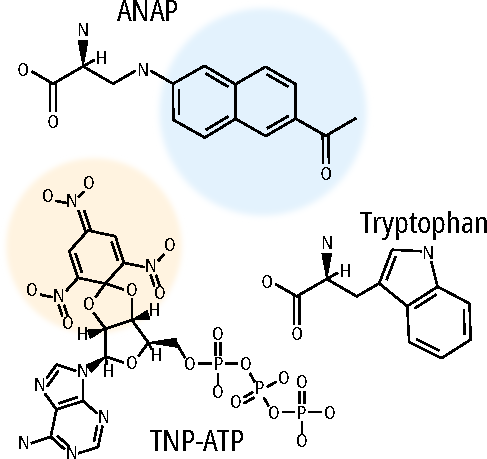
\includegraphics[width=\textwidth]{chemical_structures.pdf}
	\end{subfigure}
	\hfill
	\parbox[t]{0.5\textwidth}{
	\begin{subfigure}[t]{0.5\textwidth}
		\caption{}\label{ch3fig:spectral_overlap}
		\centering
		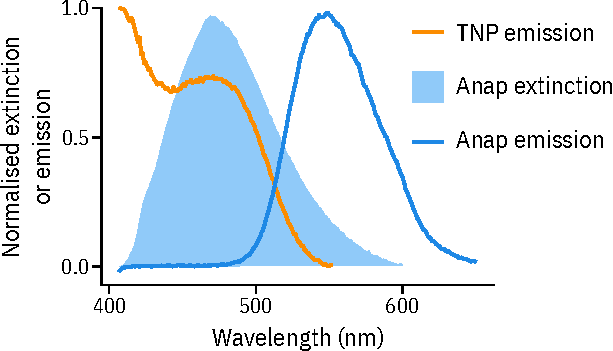
\includegraphics[width=\textwidth]{spectral_overlap.pdf}
	\end{subfigure}
	\hfill
	\begin{subfigure}[t]{0.5\textwidth}
		\caption{}\label{ch3fig:fret_efficiency}
		\centering
		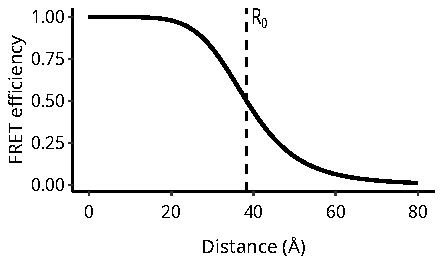
\includegraphics[width=\textwidth]{fret_efficiency.pdf}
	\end{subfigure}
	}
	\caption[ANAP and TNP-nucleotides as FRET pairs]{
		\subref{ch3fig:chemical_structures} Chemical structures of ANAP and TNP-ATP shown with the fluorescent moieties highlighted in blue (ANAP) or orange (TNP-ATP) with a tryptophan shown for reference.
		\subref{ch3fig:spectral_overlap} Normalised emission spectra (solid lines) of ANAP (blue) and TNP-nucleotides (orange) overlayed on the normalised extinction spectra of ANAP (filled light blue area).
		Extinction spectra were measured from ANAP and TNP-nucleotides separately in aqueous solution.
		ANAP emission is the averaged spectra from W311*+SUR1 expressed in unroofed membranes.
		\subref{ch3fig:fret_efficiency} Theoretical FRET efficiency displayed as a function of the distance between donor and acceptor fluorophores.
		The curve was calculated as a function of the overlap shown in \subref{ch3fig:spectral_overlap}.
		The full formula is discussed in Chapter \ref{ch:2-methods}.
	}

\end{figure}

\subsection{Choosing a site to incorporate ANAP}

The theoretical R0 of \SI{38.4}{\angstrom} for FRET between ANAP and TNP-ATP allowed for flexibility when choosing a site to incorporate ANAP.
Ideally, a residue should be chosen to maximise the following aims:

\begin{enumerate}
	\item The incorporated ANAP needs to be close enough to the nucleotide binding site of interest to report a quantifiable change in FRET when TNP-ATP is bound.
	This would not have to be close enough for \SI{100}{\percent} FRET to occur, but the greater the efficiency achieved the higher the signal-to-noise ratio would be for measuring binding.
	\item It also needs to be far enough from each other class of nucleotide binding site to avoid quenching by TNP-ATP bound to other sites.
	\item In addition to avoiding interference from other classes of binding site, we also need to avoid cross-talk between nucleotide binding sites of the same class on different subunits, as this would lead to difficulty interpreting the measured quenching.
	The ideal theoretical solution would be labelling only one nucleotide binding site per ion channel, but without using a concatemer this is not so easy in practice.
	\item More practically, incorporation of ANAP should not lead to drastic changes in nucleotide binding or channel gating properties, and the complete K\ATP{} channel needs to be expressed on the cell surface membrane.
\end{enumerate}

To narrow down which residues could be candidates for ANAP incorporation to measure binding at Kir6.2, we took three cryo-EM structures of K\ATP{} with ATP bound and computationally docked TNP-ATP into the nucleotide binding pocket (Figure \ref{ch3fig:docking}).
To assess the validity of computationally docking a ligand to each structure, we first attempted to dock ATP into the inhibitory binding pocket of Kir6.2 to check that the highest-scoring binding poses were similar to those observed in the cryo-EM structures.
Docking ATP to both \#6C3P and \#6C3O yielded binding poses which were very similar to the pose found in the cryo-EM structures (Figures \ref{ch3fig:6c3p_docking}, \ref{ch3fig:6c3o_docking}).
However, docking ATP to \#6BAA resulted in binding poses which were in a flipped orientation relative to the pose found in the cryo-EM structure (Figure \ref{ch3fig:6baa_docking}).

We then took TNP-nucleotide structures from eleven different X-ray diffraction and cryo-EM structures published on RCSB to dock to the Kir6.2 binding site of K\ATP{}.
For both \#6BAA and \#6C3P we observed that the three highest scoring binding poses for TNP-nucleotides closely resemble those of the ATP solved in complex with the channel (Figures \ref{ch3fig:6baa_docking}, \ref{ch3fig:6c3p_docking}).
It is not so clear for \#6C3O, for which the highest scoring poses are not in agreement with each other or the solved structure of ATP.

Based on the predicted TNP-ATP poses for \#6BAA and \#6C3P, we could narrow down potential ANAP incorporation sites to within \SI{25}{\angstrom} of the centre of the TNP-moiety, at which distance we would expect to see over \SI{90}{\percent} FRET efficiency when TNP-ATP is bound to Kir6.2.
In addition, we excluded residues which fell within \SI{45}{\angstrom} of NBS1 or NBS2, as this restricts the potential FRET between TNP-ATP bound at these sites and our chosen residue to roughly \SI{25}{\percent} or less.
While we can exclude residues which fall too close to the NBS's of SUR1, the close proximity of the Kir6.2 nucleotide binding sites to each other means that we cannot exclude intersubunit FRET occuring; i.e. TNP-ATP binding to a neighbouring subunit will also be able to quench ANAP to a certain extent. However, this occurs in a predictable way that we can measure and account for.

We ended up with one residue which fulfilled these criteria and for which surface membrane expression of the ANAP-incorporated channel could be detected: W311.
It is a bulky hydrophobic residue similar to ANAP, and at the time of the construct design I was not aware of mutations at this residue which had been previously identified to alter K\ATP{} function.
During the writing of this thesis, I came across an experiment by \textcite{cukras_structural_2002}, in which they mutated W311 to an alanine and were unable to observe K\ATP{} currents in excised patches.
It was not resolved whether this was an assembly, trafficking, or functional disruption.
However, as we were able to see K\ATP{} membrane expression and currents when we mutated W311 to ANAP, it is possible that this more conservative substitution is enough to overcome the lack of currents seen in the W311A mutant.

\begin{figure}[hbtp]
	\centering
	\begin{subfigure}[t]{0.30\textwidth}
		\caption{}\label{ch3fig:6baa_docking}
		\centering
		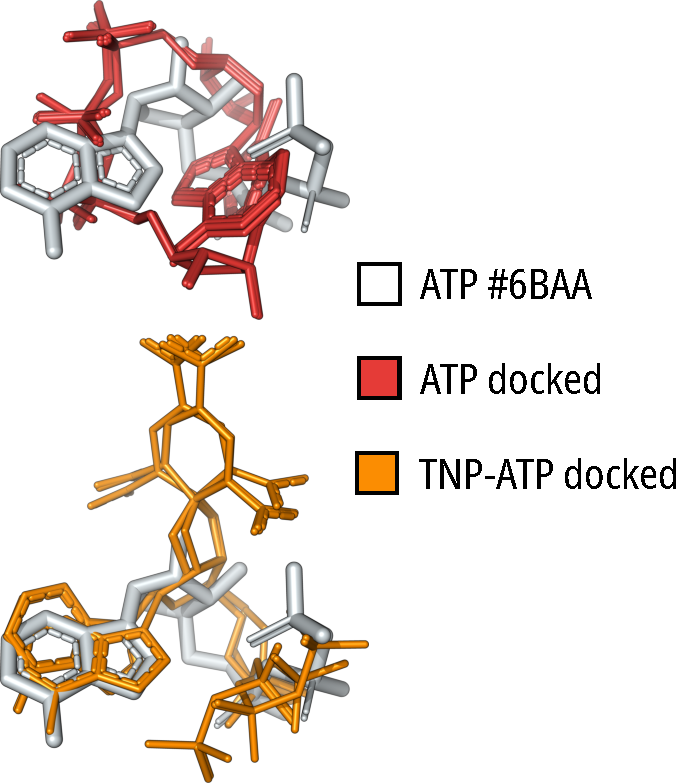
\includegraphics[width=\textwidth]{6baa_docking.pdf}
	\end{subfigure}
	\hfill
	\begin{subfigure}[t]{0.28\textwidth}
		\caption{}\label{ch3fig:6c3p_docking}
		\centering
		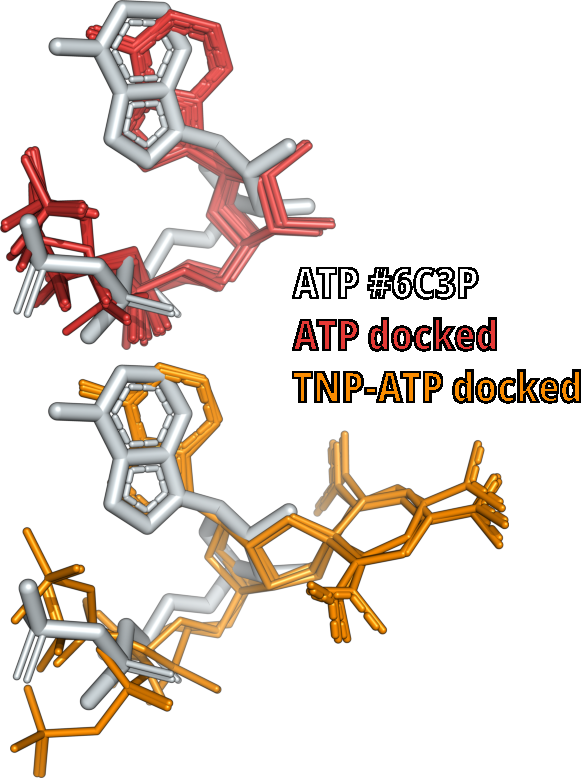
\includegraphics[width=\textwidth]{6c3p_docking.pdf}
	\end{subfigure}
	\hfill
	\begin{subfigure}[t]{0.30\textwidth}
		\caption{}\label{ch3fig:6c3o_docking}
		\centering
		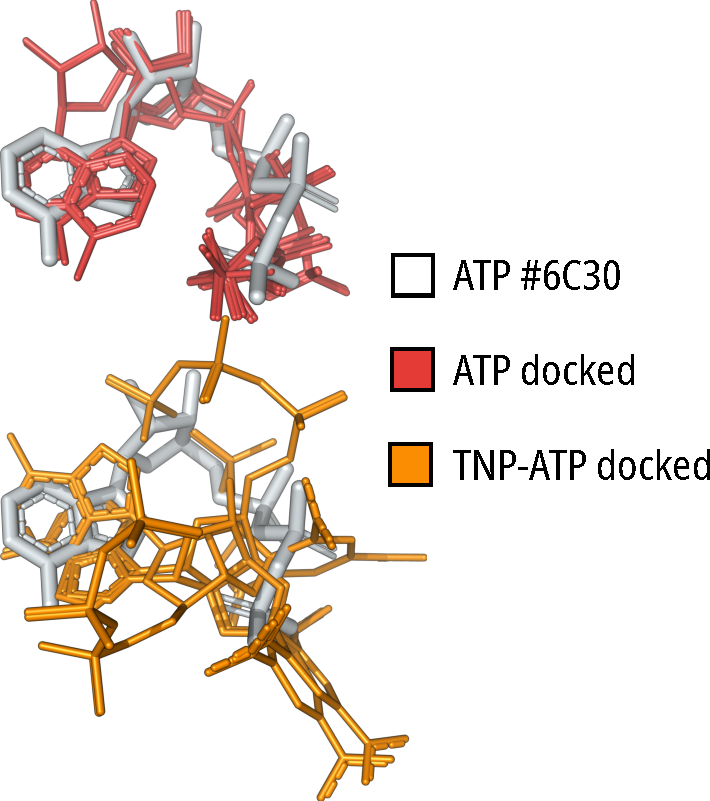
\includegraphics[width=\textwidth]{6c3o_docking.pdf}
	\end{subfigure}
	\vfill
	\begin{subfigure}[t]{0.4\textwidth}
		\caption{}\label{ch3fig:6c3p_bound}
		\centering
		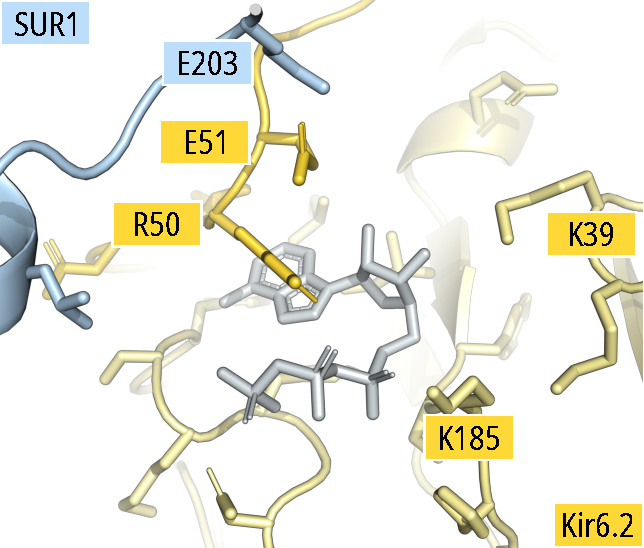
\includegraphics[width=\textwidth]{6c3p_site_bound_2.pdf}
	\end{subfigure}
	\hfill
	\begin{subfigure}[t]{0.4\textwidth}
		\caption{}\label{ch3fig:6c3p_docked}
		\centering
		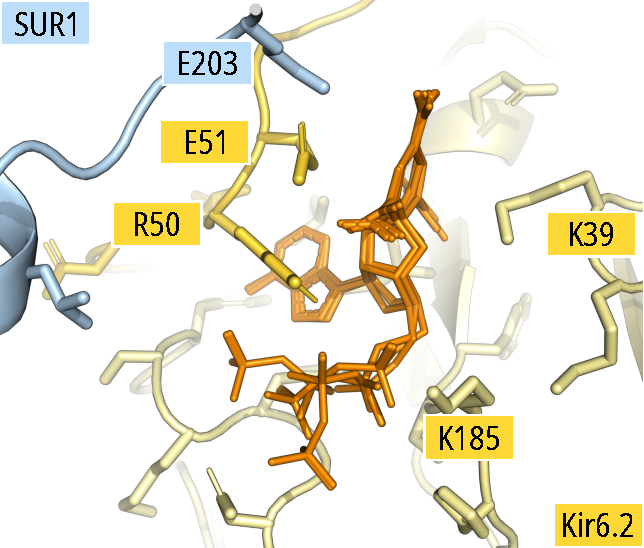
\includegraphics[width=\textwidth]{6c3p_site_docked_2.pdf}
	\end{subfigure}
	
	\caption[TNP-ATP is predicted to bind with a similar pose to ATP]{
	\subref{ch3fig:6baa_docking}, \subref{ch3fig:6c3p_docking}, \subref{ch3fig:6c3o_docking} Cryo-EM binding poses for ATP bound to Kir6.2 (white) from PDB \#6BAA (\subref{ch3fig:6baa_docking}), \#6C3P (\subref{ch3fig:6c3p_docking}) and \#6C30 (\subref{ch3fig:6c3o_docking}) overlayed with either the ten highest scoring computationally docked ATP poses (red) or the three highest scoring computationally docked TNP-ATP poses (orange) to demonstrate the similarity in binding poses.
	Starting poses for ATP were generated from ten different random seeds based on the cryo-EM poses.
	Starting poses for TNP-ATP were generated from eleven structures taken from the RCSB database for different proteins solved in the presence of TNP-ATP - the poses shown are from \#5SVQ (X-ray diffraction structure of TNP-ATP bound to the human P2X3 ion channel).
	\subref{ch3fig:6c3p_bound}, \subref{ch3fig:6c3p_docked} Cryo-EM structure of the nucleotide binding site in the presence of ATP from PDB \#6C3P (\subref{ch3fig:6c3p_bound}) or with the three highest scoring computationally docked TNP-ATP poses (\subref{ch3fig:6c3p_docked}).
	Side chains from two residues implicated in ATP binding are labelled (R50, K185), along with two residues predicted to lie within \SI{3}{\angstrom} of the TNP-moiety of the docked TNP-ATP (E51, K39).
	Residue E203 from the L0 loop of SUR1 is also labelled as it is predicted to be the closest residue on SUR1 to the TNP-moiety at a distance of \SI{5.3}{\angstrom} at the closest point.
	}\label{ch3fig:docking}
\end{figure}

\section{Incorporating ANAP into the Kir6.2 binding site}

\subsection{The Amber stop codon expression system}

ANAP can be introduced into a protein of interest by essentially expanding the genetic code to incorporate a noncanconical amino acid \cite{chin_expanding_2017}.
The Amber stop codon (TAG) is the least frequently occuring stop codon in eukaryotic cells \cite{cridge_eukaryotic_2018}, and can be repurposed to encode ANAP.
This requires the introduction of two new components into the translational machinery of the chosen heterologous expression system:
\begin{itemize}
\item A transfer RNA (tRNA) which specifically recognises the TAG codon.
\item An aminoacyl-tRNA synthetase (aaRS) which selectively attaches ANAP to the introduced tRNA \cite{lee_genetic_2009, chatterjee_genetically_2013}.
\end{itemize}

\textcite{lee_genetic_2009} used directed evolution to develop a tRNA/aaRS pair to encode ANAP in \textit{Saccharomyces cerevisiae} \cite{lee_genetic_2009}.
Briefly, they altered the specificity of \textit{Escherichia coli} leucyl-tRNA synthetase so that it was able to aminoacylate the leucyl-tRNA with ANAP, and not endogenous amino acids.
The coevolved tRNA/aaRS pair were built into an expression plasmid pANAP (Figure \ref{ch3fig:amber_codon}) which is capable of driving expression in mammalian cells \cite{chatterjee_genetically_2013}.
HEK293 cells transfected with pANAP and a plasmid encoding GFP with an Amber stop codon at residue position 40 exhibited green fluorescence only when incubated in the presence of ANAP in the culture media \cite{chatterjee_genetically_2013}, demonstrating that ANAP can be selectively incorporated into proteins in mammalian cells.

As far as we are aware, only two other studies have incorporated unnatural amino acids into Kir6.2 \cite{zhang_conserved_2015, devaraneni_structurally_2015}.
\textcite{zhang_conserved_2015} incorporated three unnatural tryptophan variants at position W68 to highlight the necessity of a planar amino acid side-chain at this location to maintain physiological K\ATP{} channel function \cite{zhang_conserved_2015}.
However, in this study \textit{Xenopus} oocytes were the heterologous expression system, so rather than transfecting a combination of plasmids, the authors injected a combination of transcribed mRNAs.

\textcite{devaraneni_structurally_2015} incorporated azidophenylalanine (AzF) at three different positions on the N-terminus of Kir6.2 (residue numbers 12, 18 and 52) \cite{devaraneni_structurally_2015}.
AzF is photocross-linkable upon exposure to UV light, and the authors used this phenomenon to investigate the extent of physical interactions between the N-terminus of Kir6.2 and SUR1, and how these interactions are mediated by pharmacological chaperones.
In this study, COSm6 cells were the heterologous expression system, and expression of AzF containing constructs was found to be dramatically reduced when compared to wild-type channels.

\subsection{ANAP incorporation into Amber stop codon containing constructs}

\begin{figure}[hbtp]
	\centering
	\begin{subfigure}[t]{0.9\textwidth}
		\caption{}\label{ch3fig:amber_codon}
		\centering
		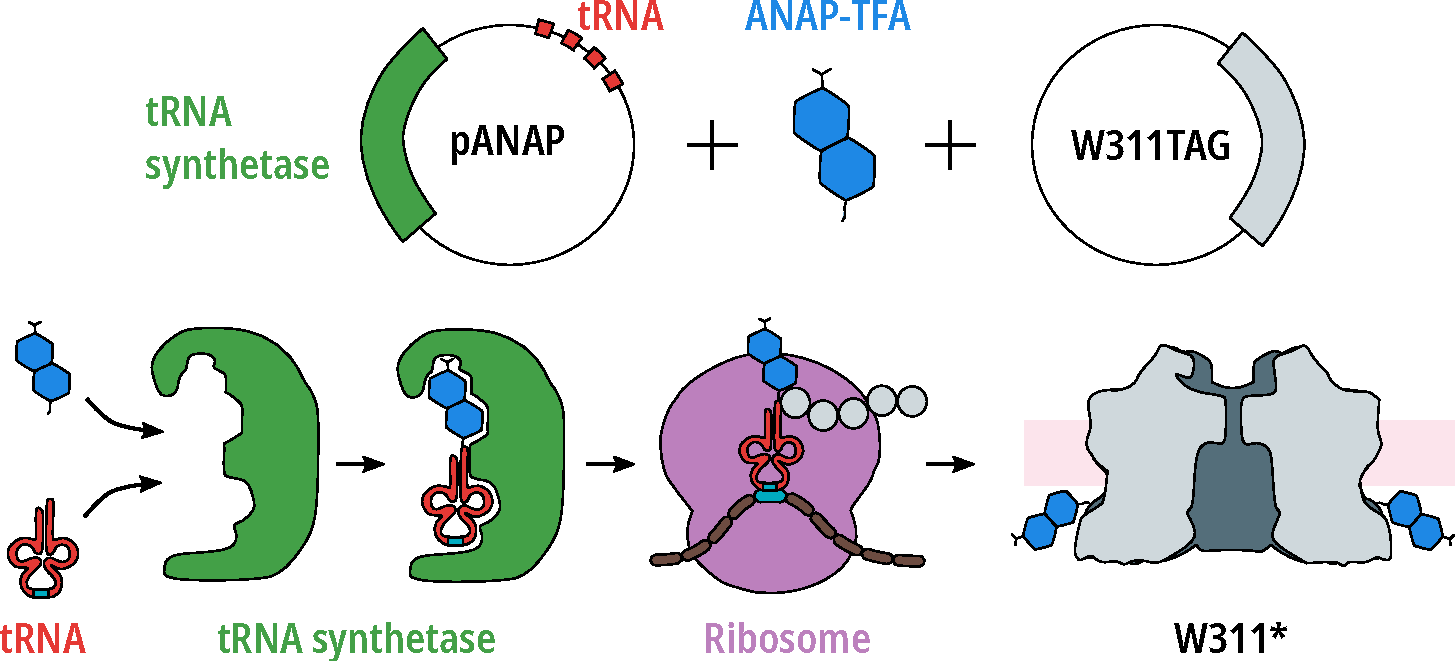
\includegraphics[width=\textwidth]{amber_codon.pdf}
	\end{subfigure}
	\vfill
	\begin{subfigure}[t]{0.25\textwidth}
		\caption{}\label{ch3fig:western_1}
		\centering
		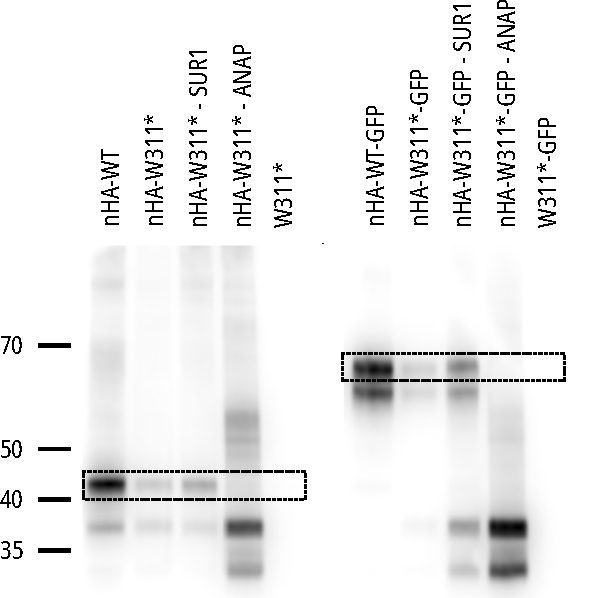
\includegraphics[width=\textwidth]{western_1.pdf}
	\end{subfigure}
	\hfill
	\begin{subfigure}[t]{0.25\textwidth}
		\caption{}\label{ch3fig:western_1b}
		\centering
		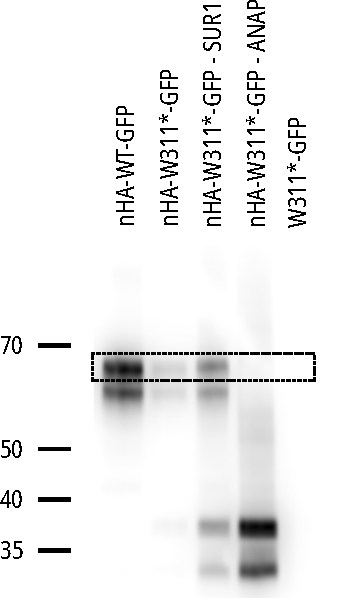
\includegraphics[width=\textwidth]{western_1b.pdf}
	\end{subfigure}
	\hfill
	\begin{subfigure}[t]{0.4\textwidth}
		\caption{}\label{ch3fig:western_2}
		\centering
		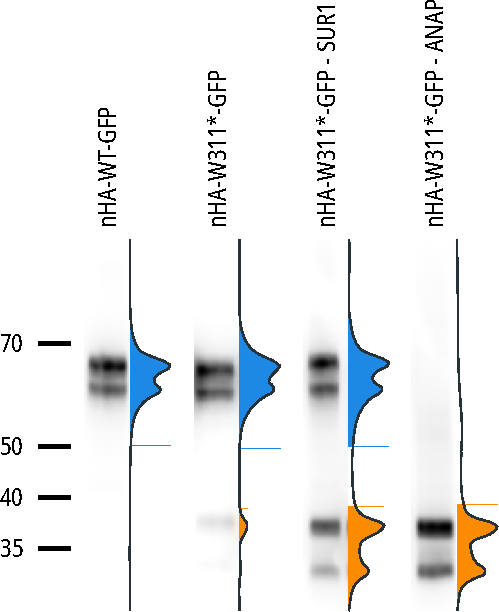
\includegraphics[width=\textwidth]{western_2.pdf}
	\end{subfigure}
	\caption[ANAP incorporation]{
	\subref{ch3fig:amber_codon} ANAP incorporation is accomplished through the transfection of two plasmids.
	pANAP codes for tRNA (red) and it's tRNA synthetase (green), while W311TAG codes for Kir6.2 with an Amber stop codon (TAG) inserted in place of the codon for W311 (grey).
	When the transfected cells are incubated with ANAP (present here as its free acid, ANAP-TFA, blue) the tRNA synthetase assembles tRNA which is capable of recognising the Amber stop codon and loads it with ANAP.
	During translation of W311TAG, the primed ANAP tRNAs recognise the TAG and insert ANAP into the desired location.
	\subref{ch3fig:western_1}, \subref{ch3fig:western_1b} Two separate western blots against the N-terminal HA epitope incorporated into WT or W311* (\subref{ch3fig:western_1}) and WT-GFP or W311*-GFP (\subref{ch3fig:western_1b}) constructs.
	Cells were co-transfected with pANAP, eRF1-E55D, and SUR1 unless otherwise indicated.
	Full-length Kir6.2 constructs are indicated on each gel with a dashed box.
	The higher molecular weight doublets represent full-length protein and an N-terminally truncated product decribed in the methods.
	\subref{ch3fig:western_2} Each lane from the gel containing C-terminally GFP-tagged constructs in \subref{ch3fig:western_1b} is displayed normalised to its highest intensity accompanied by the line averaged density trace.
	The density peak corresponding to full-length and N-terminally truncated Kir6.2 is filled in blue.
	The density peak for C-terminally truncated and doubly truncated Kir6.2 is filled in orange.
	}\label{ch3fig:anap_incorporation}
\end{figure}

The nature of the amber stop codon suppression system requires a number of careful controls to ensure the following:

\begin{enumerate}
	\item Stop codon recognition is not perfect, and there is a chance of read-through.
	Instead of incorporating ANAP, it is possible that the translation machinery can insert endogenous amino acids instead, leading to production of full length,unlabelled Kir6.2.
	However, we found that cells transfected with W311TAG constructs and pANAP which were not cultured in the presence of ANAP did not produce full length Kir6.2 (Figure \ref{ch3fig:western_1}, \ref{ch3fig:western_1b}, \ref{ch3fig:western_2}), suggesting there is minimal read-through of the stop codon in our experiments.
	\item Introducing a stop codon creates a risk that truncated Kir6.2 will be produced instead of ANAP labelled Kir6.2.
	This risk can be reduced by transfecting a dominant negative engineered version of eukaryotic translation termination factor 1(eRF1-E55D), which does not efficiently terminate protein synthesis in response to the amber stop codon (but leaves opal and ochre stop codons nearly unaffected) and thus increases the incorporation of ANAP \cite{schmied_efficient_2014}.
	We found that transfection of W311TAG constructs with a C-terminal GFP tag produced minimal truncated Kir6.2 (less than \SI{10}{\percent} of the total density observed in Figure \ref{ch3fig:western_2}).
	\item Despite being the least frequent eukaryotic stop codon, the amber stop codon is still present in a significant number of protein sequences.
	We must be careful that ANAP is not incorporated into a protein which localises to the plasma membrane to an extent which would affect our ability to assign ANAP fluorescence to Kir6.2.
	We found that in cells transfected with GFP-tagged Kir6.2 without an amber stop codon, there was no increase in ANAP fluorescence at the cell membrane (Figure \ref{ch3fig:wt_confocal}, \ref{ch3fig:wt_confocal_profiles}).
	By contrast, when W311TAG-GFP was transfected, we saw a clear increase in ANAP fluorescence at the cell membrane (Figure \ref{ch3fig:w311_confocal}, \ref{ch3fig:w311_confocal_profiles}), suggesting that any observed ANAP fluorescence at the cell membrane originates from our labelled Kir6.2 construct.
\end{enumerate}

\begin{figure}[hbtp]
	\centering
	\begin{subfigure}[t]{0.55\textwidth}
		\caption{}\label{ch3fig:wt_confocal}
		\centering
		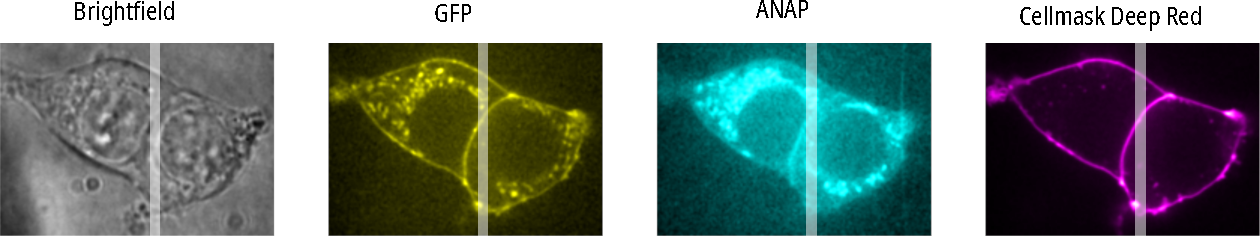
\includegraphics[width=\textwidth]{wt_confocal.pdf}
	\end{subfigure}
	\hfill
	\begin{subfigure}[t]{0.35\textwidth}
		\caption{}\label{ch3fig:wt_confocal_profiles}
		\centering
		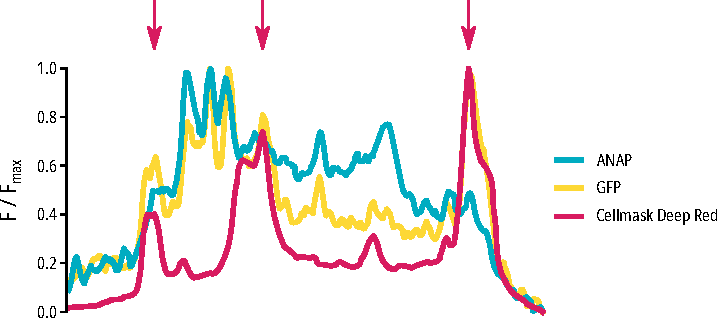
\includegraphics[width=\textwidth]{wt_confocal_profiles.pdf}
	\end{subfigure}
	\vfill
	\begin{subfigure}[t]{0.55\textwidth}
		\caption{}\label{ch3fig:w311_confocal}
		\centering
		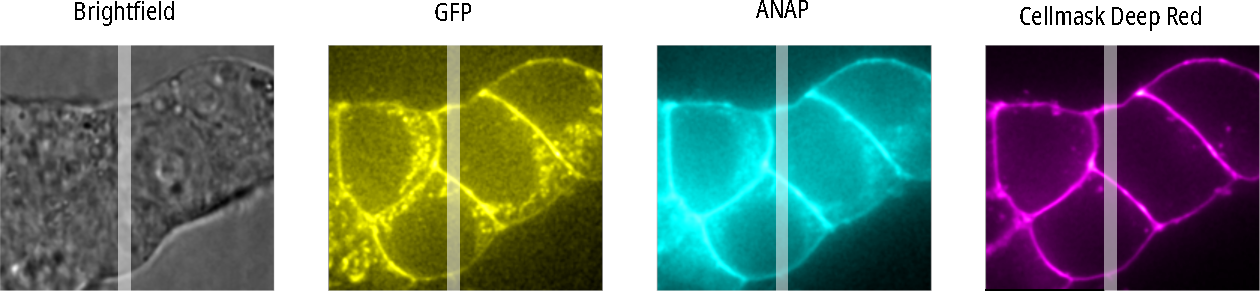
\includegraphics[width=\textwidth]{w311_confocal.pdf}
	\end{subfigure}
	\hfill
	\begin{subfigure}[t]{0.35\textwidth}
		\caption{}\label{ch3fig:w311_confocal_profiles}
		\centering
		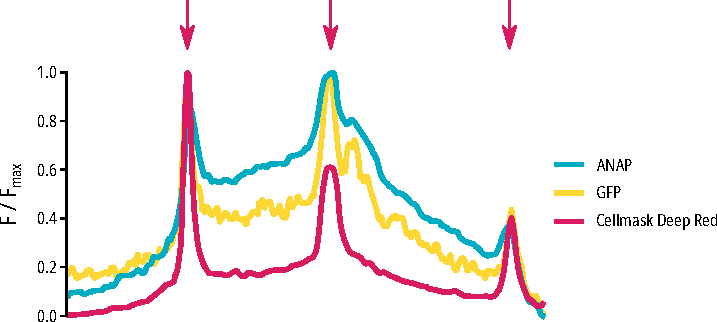
\includegraphics[width=\textwidth]{w311_confocal_profiles.pdf}
	\end{subfigure}
	\caption[Confocal imaging]{
	\subref{ch3fig:wt_confocal}, \subref{ch3fig:w311_confocal} Confocal images of two HEK293T cells transfected with WT-GFP (\subref{ch3fig:wt_confocal}) or W311TAG-GFP (\subref{ch3fig:w311_confocal}), plus SUR1, pANAP, peRF1-E55D and with ANAP in the culture medium.
	Cells were incubated with Cellmask Deep Red for ten minutes before imaging to label the plasma membranes.
	The vertical grey box indicates the section of the images plotted in \subref{ch3fig:wt_confocal_profiles} and \subref{ch3fig:w311_confocal_profiles}.
	Images are displayed after median filtering with a box radius of 5, and normalising the intensities per channel.
	\subref{ch3fig:wt_confocal_profiles}, \subref{ch3fig:w311_confocal_profiles} The line-averaged intensity of the pixels in the grey boxes in \subref{ch3fig:wt_confocal} and \subref{ch3fig:w311_confocal} respectively.
	The plasma membranes are identifiable as clear peaks in the Cellmask Deep Red fluorescence (magenta) and are marked with arrows.
	Notably, while there are clear GFP peaks at the membrane in both \subref{ch3fig:wt_confocal_profiles} and \subref{ch3fig:w311_confocal_profiles}, only in \subref{ch3fig:w311_confocal_profiles} do peaks in the ANAP fluorescence coincide with the membrane.
	}
\end{figure}

\section{Testing for functional membrane expression}

\subsection{Surface expression of HA-epitope labelled Kir6.2 constructs}

To assess the ability of ANAP-incorporating constructs to traffic to the plasma membrane, we used a luminescence-based surface expression assay \cite{zerangue_new_1999}.
This assay relies on the recognition of a human influenza hemagglutinin (HA)-epitope introduced into an extracellular region of the protein of interest (in this case, the N-terminal region of Kir6.2) by an anti-HA primary antibody followed by a horseradish peroxidase (HRP)-conjugated secondary antibody.
The luminescence after applying HRP substrate is then proportional to the amount of protein at the plasma membrane of the cells.

We assessed the membrane expression of N-terminally HA-tagged Kir6.2 (WT-HA) in the presence or absence of ANAP in the culture media and in the presence or absence of cotransfected SUR1.
We also measured how the addition of a C-terminal GFP tag affected membrane expression under these conditions.
We used untagged Kir6.2 as a control for nonspecific luminescence.

We found that for wild-type Kir6.2 (WT) there is roughly a 20-fold increase over background in observed luminescence when coexpressed with SUR1, and roughly a 100-fold increase for the C-terminally GFP tagged Kir6.2 (WT-GFP, Figure \ref{ch3fig:surface_expression_1}, \ref{ch3fig:surface_expression_3}).
There is no difference in surface expression of these constructs when ANAP is present in the culture medium (Figure \ref{ch3fig:surface_expression_1}, \ref{ch3fig:surface_expression_4}).
When ANAP is incorporated at either residue 183 or 311 (F183* and W311* respectively, F183* included here as an example of a construct deemed unsuitable for further experiments) we see an increase over background in luminescence when coexpressed with SUR1 and with ANAP present in the culture medium (Figure \ref{ch3fig:surface_expression_1}, \ref{ch3fig:surface_expression_3}).
The presence of the C-terminal GFP tag increases luminescence further for both constructs, dramatically so for W311*.
However, when F183* is transfected and ANAP is not present in the culture media we still see a similar increase in fluorescence over background when compared to the luminescence when ANAP is present (Figure \ref{ch3fig:surface_expression_1}, \ref{ch3fig:surface_expression_4}), suggesting that a large proportion of the protein reaching the cell surface membrane does not have ANAP incorporated.
In contrast, when W311*-GFP is transfected with SUR1 in the presence of ANAP, we see a 10-fold increase in luminescence compared to when ANAP is not present, consistent with the majority of cell surface expressed protein having incorporated ANAP.
We also see a consistent increase in luminescence for all constructs aside from W311* when cotransfected with SUR1 (Figure \ref{ch3fig:surface_expression_2}), suggesting that the incorporation of ANAP and the addition of a C-terminal GFP tag do not affect the role of SUR1 in forming the full K\ATP{} complex and trafficking to the cell surface membrane.

\begin{figure}[hbtp]
	\centering
	\begin{subfigure}[t]{0.45\textwidth}
		\caption{}\label{ch3fig:surface_expression_1}
		\centering
		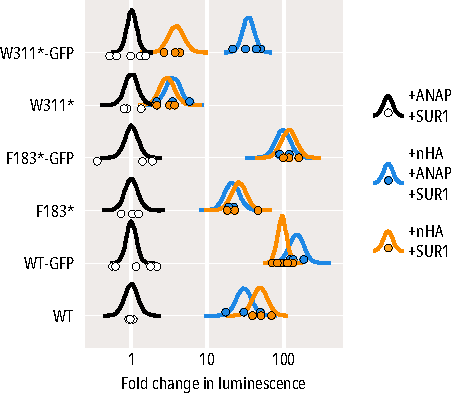
\includegraphics[width=\textwidth]{surface_expression_1.pdf}
	\end{subfigure}
	\hfill
	\begin{subfigure}[t]{0.45\textwidth}
		\caption{}\label{ch3fig:surface_expression_2}
		\centering
		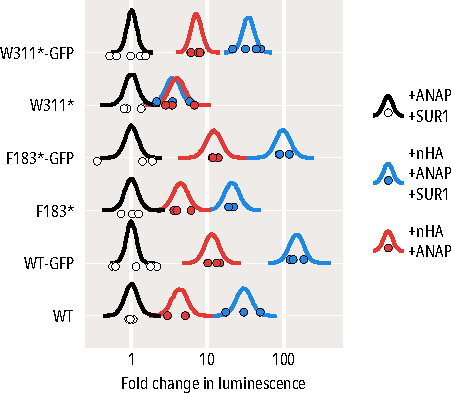
\includegraphics[width=\textwidth]{surface_expression_2.pdf}
	\end{subfigure}
	\vfill
	\begin{subfigure}[t]{0.45\textwidth}
		\caption{}\label{ch3fig:surface_expression_3}
		\centering
		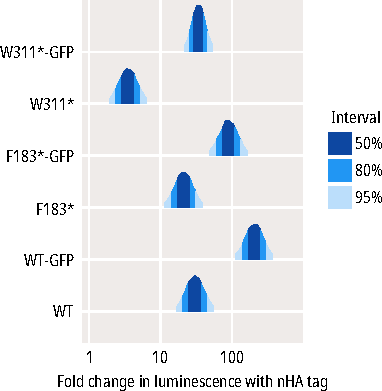
\includegraphics[width=\textwidth]{surface_expression_3.pdf}
	\end{subfigure}
	\hfill
	\begin{subfigure}[t]{0.45\textwidth}
		\caption{}\label{ch3fig:surface_expression_4}
		\centering
		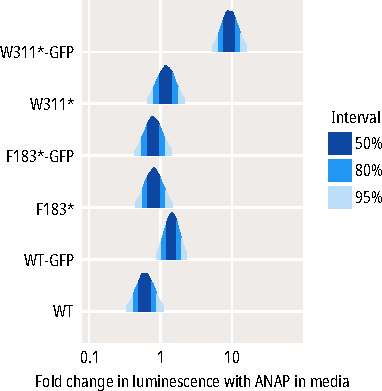
\includegraphics[width=\textwidth]{surface_expression_4.pdf}
	\end{subfigure}
	\caption[ANAP construct surface expression assay]{
	\subref{ch3fig:surface_expression_1}, \subref{ch3fig:surface_expression_2} Each point represents a luminescence reading from one well of a 6-well plate.
	The coloured curves are the posterior probability distributions for surface expression of Kir6.2 constructs derived from those readings as described in the methods.
	Before fitting, the observations for each construct were centered by subtracting the mean of the luminesence observed without the N-terminal HA tag.
	Observations for constructs without the N-terminal HA tag and for constructs transfected with both ANAP and SUR1 are duplicated between panels to clarify the differences observed when either ANAP (\subref{ch3fig:surface_expression_1}) or SUR1 (\subref{ch3fig:surface_expression_2}) are omitted.
	\subref{ch3fig:surface_expression_3}, \subref{ch3fig:surface_expression_4} Contrasts between constructs differing only in the presence or absence of the N-terminal HA-tag (\subref{ch3fig:surface_expression_3}) or the presence or absence of ANAP in the culture media (\subref{ch3fig:surface_expression_4}).
	Different credible intervals in the posterior probability distribution of the contrasts are shown in shades of blue.
	Only W311*-GFP coexpressed with SUR1 shows a large fold change in luminescence when ANAP is included in the culture media.
	}
\end{figure}

\subsection{Electrophysiology of Kir6.2 constructs}

To establish whether W311*-GFP formed K\ATP{} channels with similar function to wild-type, we excised patches from cells transfected with either WT-GFP or W311*-GFP cotransfected with SUR1.
Excision was performed in Mg\textsuperscript{2+}-free solution to reduce rundown and to prevent activation of the channel by nucleotides.
We observed similar magnitudes of current for both WT-GFP and W311*-GFP, and the currents ran down at similar rates.

We fit our inhibition data with equation \ref{eq:hill} (Figure \ref{ch3fig:atp_inhibition_1}) as described in the methods.
Briefly, our fitting procedure assumes that there is a population parameter for $IC_{50}$, $I_{max}$ and $h$, and an additional 'random' effect on $IC_{50}$ that can differ between experiments (shown in Figure \ref{ch3fig:atp_inhibition_2}).
Our fits result in posterior probability distributions for the population $IC_{50}$ parameter shown in blue in Figure \ref{ch3fig:ec50_fits_1}.
These distributions reflect our confidence in the population parameter for the $IC_{50}$.
For all $IC_50$ and $EC_{50}$ values fitted this way, in the text we will report the \SI{95}{\percent} credible intervals of the posterior probability distribution for the fitted population parameter.

Perfusion of ATP resulted in current inhibition with an IC\textsubscript{50} of \SIrange{24}{45}{\micro\Molar} for WT-GFP+SUR1 and \SIrange{75}{124}{\micro\Molar} for W311*-GFP+SUR1.
Thus, despite the distance from the ATP binding site, the incorporation of ANAP at W311 clearly affects some aspect of nucleotide inhibition.
However, we assume that insights into the function of the ANAP-incorporating channel will still be applicable to wild-type channels despite the change in nucleotide inhibition.

Next, we established that TNP-ATP inhibits K\ATP{} (Figure \ref{ch3fig:tnpatp_inhibition_1}, \ref{ch3fig:tnpatp_inhibition_2}).
We observed current inhibition with an IC\textsubscript{50} of \SIrange{0.7}{1.8}{\micro\Molar} for WT-GFP+SUR1 and \SIrange{2.9}{10}{\micro\Molar} for W311*-GFP+SUR1.
K\ATP{} thus appears to be more sensitive to inhibition by TNP-ATP than by ATP.
This could potentially be due to extra contacts made by the TNP moiety with Kir6.2, seen in our computational docking (Figure \ref{ch3fig:docking}).

\begin{figure}[hbtp]
	\centering
	\begin{subfigure}[t]{0.45\textwidth}
		\caption{}\label{ch3fig:atp_inhibition_1}
		\centering
		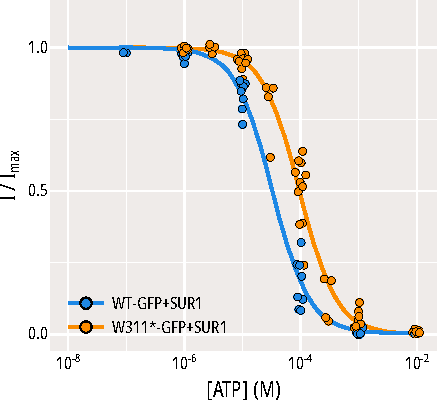
\includegraphics[width=\textwidth]{atp_inhibition_1.pdf}
	\end{subfigure}
	\hfill
	\begin{subfigure}[t]{0.45\textwidth}
		\caption{}\label{ch3fig:tnpatp_inhibition_1}
		\centering
		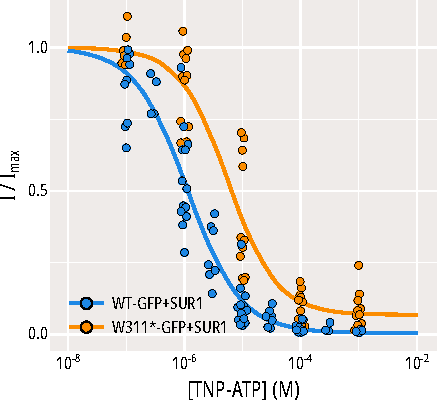
\includegraphics[width=\textwidth]{tnpatp_inhibition_1.pdf}
	\end{subfigure}
	\vfill
	\begin{subfigure}[t]{0.9\textwidth}
		\caption{}\label{ch3fig:atp_inhibition_2}
		\centering
		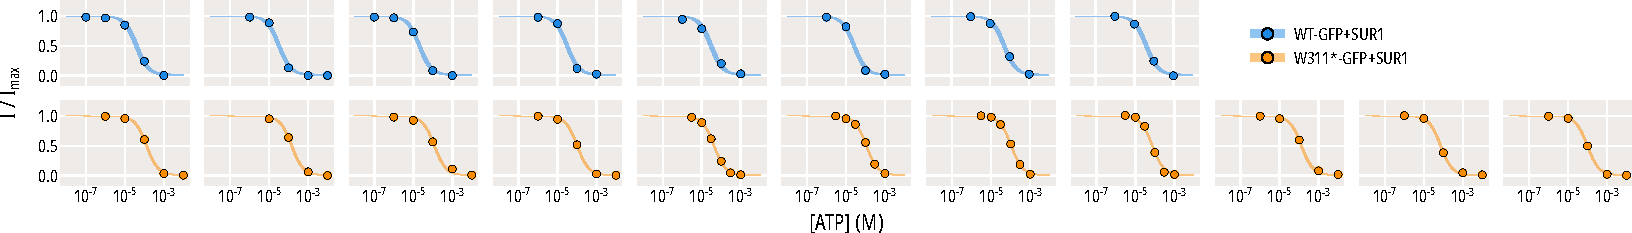
\includegraphics[width=\textwidth]{atp_inhibition_2.pdf}
	\end{subfigure}
	\vfill
	\begin{subfigure}[t]{0.9\textwidth}
		\caption{}\label{ch3fig:tnpatp_inhibition_2}
		\centering
		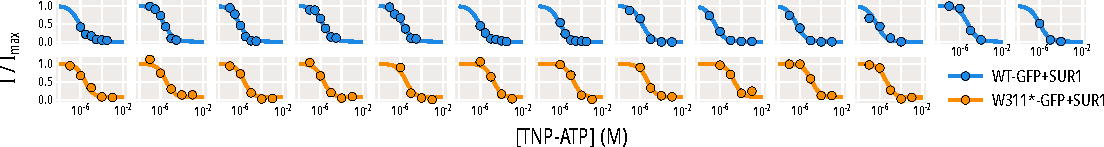
\includegraphics[width=\textwidth]{tnpatp_inhibition_2.pdf}
	\end{subfigure}
	\vfill
	\begin{subfigure}[t]{0.6\textwidth}
		\caption{}\label{ch3fig:ec50_fits_1}
		\centering
		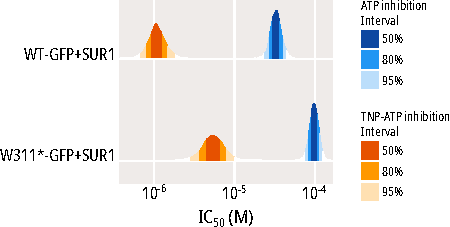
\includegraphics[width=\textwidth]{ec50_fits_1.pdf}
	\end{subfigure}
	\caption[WT-GFP and W311*-GFP electrophysiology]{
	\subref{ch3fig:atp_inhibition_1}, \subref{ch3fig:tnpatp_inhibition_1} Inhibition of current by ATP (\subref{ch3fig:atp_inhibition_1}) or TNP-ATP (\subref{ch3fig:tnpatp_inhibition_1}) in excised patches expressing either WT-GFP+SUR1 (blue) or W311*-GFP+SUR1 (orange).
	Each point represents an individual measurement at the nucleotide concentration indicated, bracketed by perfusion with nucleotide-free solution and normalised to the mean current observed there.
	The line is the median estimate and the smooth filled curves are the \SI{95}{\percent} credible intervals of the posterior probability distribution of fits to equation \ref{eq:hill} as described in the methods.
	\subref{ch3fig:atp_inhibition_2}, \subref{ch3fig:tnpatp_inhibition_2} Data from each experiment is shown separately.
	The smooth filled curves are the \SI{95}{\percent} credible intervals of the posterior predictions for each experiment.
	\subref{ch3fig:ec50_fits_1} Posterior probability distributions for the population $IC_{50}$ values for inhibition by ATP (blue) or TNP-ATP (orange).
	}
\end{figure}

\subsection{Unroofed membrane binding assay of Kir6.2 constructs}

We then directly measured nucleotide binding to W311*-GFP in unroofed membranes.
Briefly sonicating transfected cells adhered to coverslips results in the adhered lower membrane of the cell remaining stuck to the coverslip while the rest of the cell is disrupted and the contents are perfused away.
This leaves the cytoplasmic domains of expressed K\ATP{} channels accessible to TNP-ATP in the perfusate.
These patches of membrane are barely visible under brightfield illumination, but due to the presence of the C-terminal GFP tag and the incorporated ANAP, we can see patches of membrane expressing K\ATP{} channels light up when we excite either fluorophore (Figure \ref{ch3fig:unroofed_images}).
By measuring the fluorescence spectra of patches of unroofed membrane, we can separate the fluorescence emission peaks of the C-terminal GFP tag and the incorporated ANAP (Figure \ref{ch3fig:unroofed_spectral_images}).
The peak at \SI{472}{\nano\metre} corresponds to ANAP emission, while the peak at \SI{508}{\nano\metre} corresponds to GFP emission.
We observed no change in the locations of those peaks in the presence of ATP or TNP-ATP.

Perfusing TNP-ATP results in a decrease in the peak corresponding to ANAP fluorescence, and a concomittant increase in a fluorescence peak at \SI{561}{\nano\metre} which corresponds to the TNP-ATP (Figure \ref{ch3fig:unroofed_spectral_traces}).
This phenomenon is the result of FRET between TNP-ATP bound to the channel at the Kir6.2 binding site.
The decrease in ANAP fluorescence is almost directly correlated to an increase in bound nucleotide.
We chose to measure the decrease in ANAP fluorescence rather than the increase in TNP-ATP fluorescence or the change in the ratio of ANAP:TNP-ATP fluorescence as we know that the ANAP fluorescence is specific to the Kir6.2 binding site.
Increases in TNP-ATP fluorescence could in part be due to direct excitation of TNP-ATP bound to other membrane proteins.
We can plot the quenching of ANAP fluorescence as a concentration-response curve as in Figure \ref{ch3fig:unroofed_intensities}.

\begin{figure}[hbtp]
	\centering
	\begin{subfigure}[t]{0.3\textwidth}
		\caption{}\label{ch3fig:unroofed_images}
		\centering
		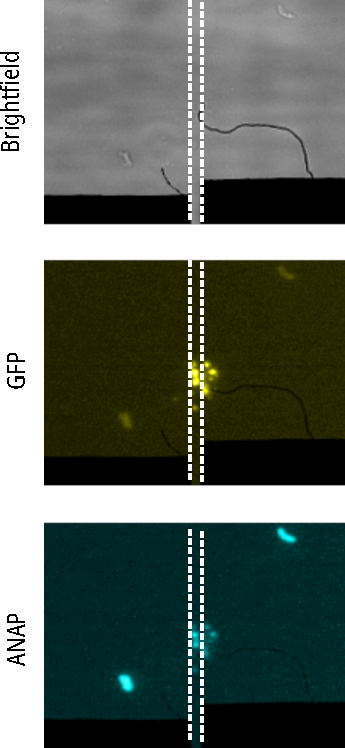
\includegraphics[width=\textwidth]{unroofed_images.pdf}
	\end{subfigure}
	\hfill
	\begin{subfigure}[t]{0.6\textwidth}
		\caption{}\label{ch3fig:unroofed_spectral_images}
		\centering
		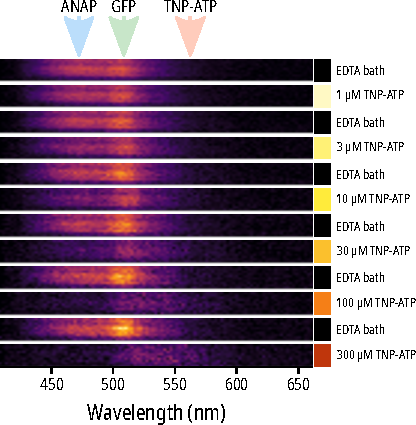
\includegraphics[width=\textwidth]{unroofed_spectral_images.pdf}
	\end{subfigure}
	\vfill
	\begin{subfigure}[t]{0.45\textwidth}
		\caption{}\label{ch3fig:unroofed_spectral_traces}
		\centering
		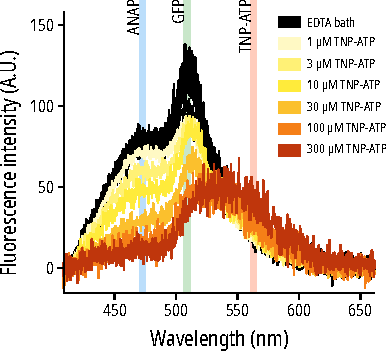
\includegraphics[width=\textwidth]{unroofed_spectral_traces.pdf}
	\end{subfigure}
	\hfill
	\begin{subfigure}[t]{0.45\textwidth}
		\caption{}\label{ch3fig:unroofed_intensities}
		\centering
		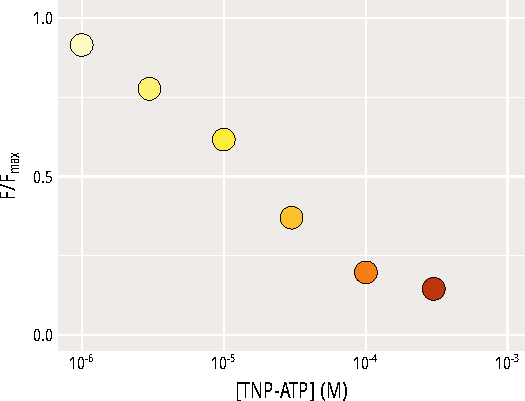
\includegraphics[width=\textwidth]{unroofed_intensities.pdf}
	\end{subfigure}
	\caption[Unroofed membranes spectral images]{
	\subref{ch3fig:unroofed_images} An unroofed membrane patch imaged either with brightfield illumination (top panel), GFP fluorescence (middle panel) or ANAP fluorescence (bottom panel).
	The dashed white lines indicate the region of the image isolated by the spectrometer mask for spectral imaging.
	\subref{ch3fig:unroofed_spectral_images} Bleaching-corrected spectral images of the unroofed membrane patch in \subref{ch3fig:unroofed_images} captured in the presence of different concentrations of TNP-ATP.
	Each image represents the region delineated by the dashed white lines in \subref{ch3fig:unroofed_images}, but the $x$-dimension is lost and instead we are able to separate the emitted light by wavelength.
	The location of the three fluorescent peaks are indicated by arrows at the top of the plot.
	\subref{ch3fig:unroofed_spectral_traces} Line-averaged, bleaching-corrected traces of the spectral images in \subref{ch3fig:unroofed_spectral_images} coloured according to the TNP-ATP concentration present.
	The two clearest peaks in emission belong to ANAP and GFP, marked with light blue and light green shaded bars respectively.
	At the higher TNP-ATP concentrations, the presence of a third peak belonging to the TNP-moiety begins to appear as the ANAP peak reduces in intensity due to FRET, marked with a light orange shaded bar.
	\subref{ch3fig:unroofed_intensities} Bleaching-corrected ANAP fluorescence intensities of the spectral traces in \subref{ch3fig:unroofed_spectral_images} expressed as the average fluorescence of the ANAP peak (the average intensity of the spectra inside the grey line in \subref{ch3fig:unroofed_spectral_images}) divided by the average fluorescence of the ANAP peak in $0$ TNP-ATP, or $F/F_{max}$.
	}
\end{figure}

Before analysis, ANAP bleaching was corrected as shown in Figure \ref{ch3fig:bleaching_plots_2}.
ANAP intensities of spectra imaged during bath perfusion with TNP-ATP free solution, in between applications of TNP-ATP, were fit with Equation \ref{eq:bleaching}.
We found that in all unroofed membrane experiments bleaching was well described by a single exponential fit to equation \ref{eq:bleaching}.
In each experiment, there was a mean value of \SI{49}{\percent} ANAP fluorescence remaining by the last exposure (Figure \ref{ch3fig:bleaching_terms_4}), means we maintained a good signal-to-noise ratio for each spectra imaged.

\begin{figure}[hbtp]
	\centering
	\begin{subfigure}[t]{0.9\textwidth}
		\caption{}\label{ch3fig:bleaching_plots_2}
		\centering
		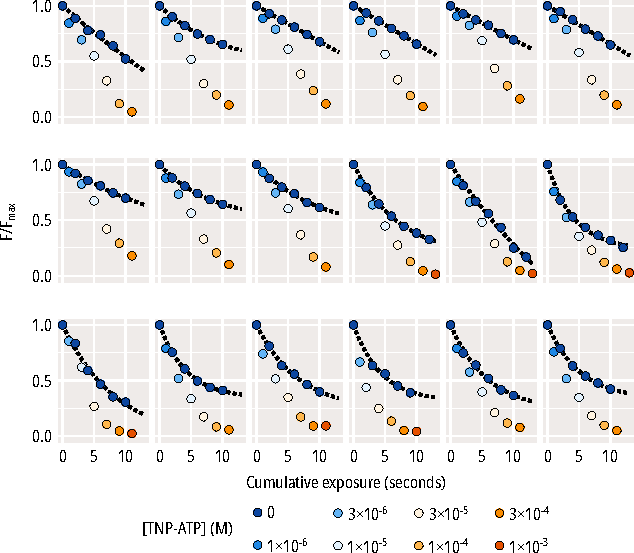
\includegraphics[width=\textwidth]{bleaching_plots_2.pdf}
	\end{subfigure}
	\vfill
	\begin{subfigure}[t]{0.45\textwidth}
		\caption{}\label{ch3fig:bleaching_terms_3}
		\centering
		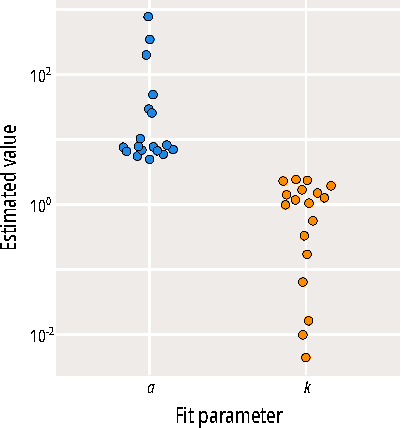
\includegraphics[width=\textwidth]{bleaching_terms_3.pdf}
	\end{subfigure}
	\hfill
	\begin{subfigure}[t]{0.45\textwidth}
		\caption{}\label{ch3fig:bleaching_terms_4}
		\centering
		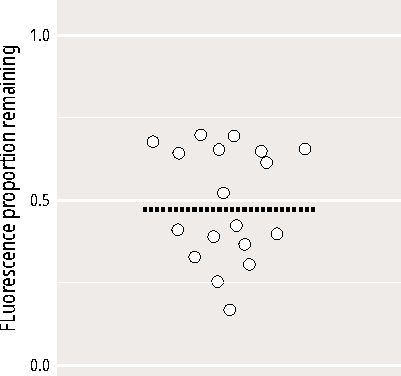
\includegraphics[width=\textwidth]{bleaching_terms_4.pdf}
	\end{subfigure}
	\caption[Unroofed membranes bleaching correction]{
	\subref{ch3fig:bleaching_plots_2} Normalised ANAP fluorescence intensities in unroofed membranes from cells expressing W311*-GFP+SUR1 perfused at different concentrations of TNP-ATP are shown as points coloured according to the concentration of TNP-ATP.
	The black dashed lines are fits to the fluorescence intensities without TNP-ATP present with equation \ref{eq:bleaching}.
	\subref{ch3fig:bleaching_terms_3} Values of the two parameters in equation \ref{eq:bleaching} for fits to each of the experiments in \subref{ch3fig:bleaching_plots_2}.
	Estimates are shown on a log scale due to a number of the experiments which show bleaching behaviour on a different timescale than the majority.
	\subref{ch3fig:bleaching_terms_4} Proportion of ANAP fluorescence remaining unbleached in the last exposure taken in the absence of TNP-ATP in each experiment.
	The dashed line is the mean, with a value of $0.49$.
	}
\end{figure}

While our measurements of ANAP quenching are proportional to nucleotide binding to K\ATP{}, the raw $F/F_{max}$ observations are not directly equivalent to the unbound fraction of Kir6.2 subunits.
This non-equivalence is due to two factors.
Firstly, there is the potential for crosstalk between ANAP incorporated in one subunit and TNP-ATP bound to the adjacent subunits.
To determine the extent to which this crosstalk would affect the measured FRET efficiency when ANAP is incorporated at position 311, we adapted a program described by \textcite{deplazes_exifret_2012} which uses a numerical method to model FRET in complex geometries.
We implemented a simple version of this program in Python which uses a Monte Carlo simulation scheme to approximate the observed FRET efficiency for a given set of donor and acceptor fluorophores and coordinates.
An overview of the program is shown in Figure \ref{ch3fig:exifret_program}.
We did not measure the fluorescence lifetimes and quantum yields of ANAP and TNP-ATP directly, instead using previously determined values \cite{zagotta_measuring_2016-1, ye_spectroscopic_1999, ishikawa_single-molecule_2002}.
The fluorescence lifetime of TNP-ATP differs when it is bound to proteins; we ran simulations using the fluorescence lifetime of TNP-ATP in solution and the fluorescence lifetime of bound TNP-ATP and saw no difference in the FRET efficiency.

We simulated the expected FRET for a single K\ATP{} channel bound to 0-4 molecules of TNP-ATP in two different scenarios.
In the idealised scenario, each ANAP molecule is only able to FRET with the TNP-ATP molecule bound at the closest inhibitory binding site (Figure \ref{ch3fig:exifret_coords}).
In the actual scenario, which resembles the experimental paradigm, each ANAP molecule is able to FRET with any bound TNP-ATP molecule in a probabilistic manner dependent on the inter-fluorophore distance.
We can observe that there is a systematic deviation in the FRET efficiency between these two scenarios (Figure \ref{ch3fig:exifret_out}), which we can correct by transforming the actual values ($F/F_{max}$) into adjusted values ($log_2(\frac{F}{F_{max} + 1})$).
This is an empirical transformation based on the observed deviation.

Secondly, we need to correct for incomplete FRET due to the distance between the donor and acceptor.
Based on the results of the computational docking, we predict a maximal FRET efficiency of \SI{91}{\percent} when a TNP-ATP molecule is bound to each Kir6.2 subunit.
Fitting our adjusted data to a Hill equation results in a maximum observed FRET efficiency ($E_{max}$) of \SI{91}{\percent}, agreeing well with our prediction.
We can then constrain our Hill fits so that $E_{max}$ is equal to this maximum FRET efficiency, so that the $EC_{50}$ parameter we obtain is equivalent to the $EC_{50}$ of TNP-ATP binding.

\begin{figure}[hbtp]
	\centering
	\begin{minipage}{0.35\textwidth}
	\begin{subfigure}[t]{\textwidth}
		\caption{}\label{ch3fig:exifret_program}
		\centering
		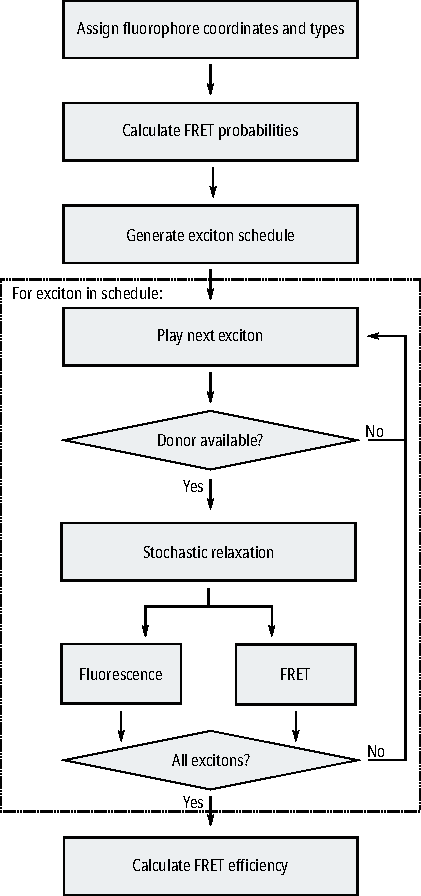
\includegraphics[width=\textwidth]{exifret_program.pdf}
	\end{subfigure}
	\end{minipage}
	\hfill
	\begin{minipage}{0.55\textwidth}
	\begin{subfigure}[t]{\textwidth}
		\caption{}\label{ch3fig:exifret_coords}
		\centering
		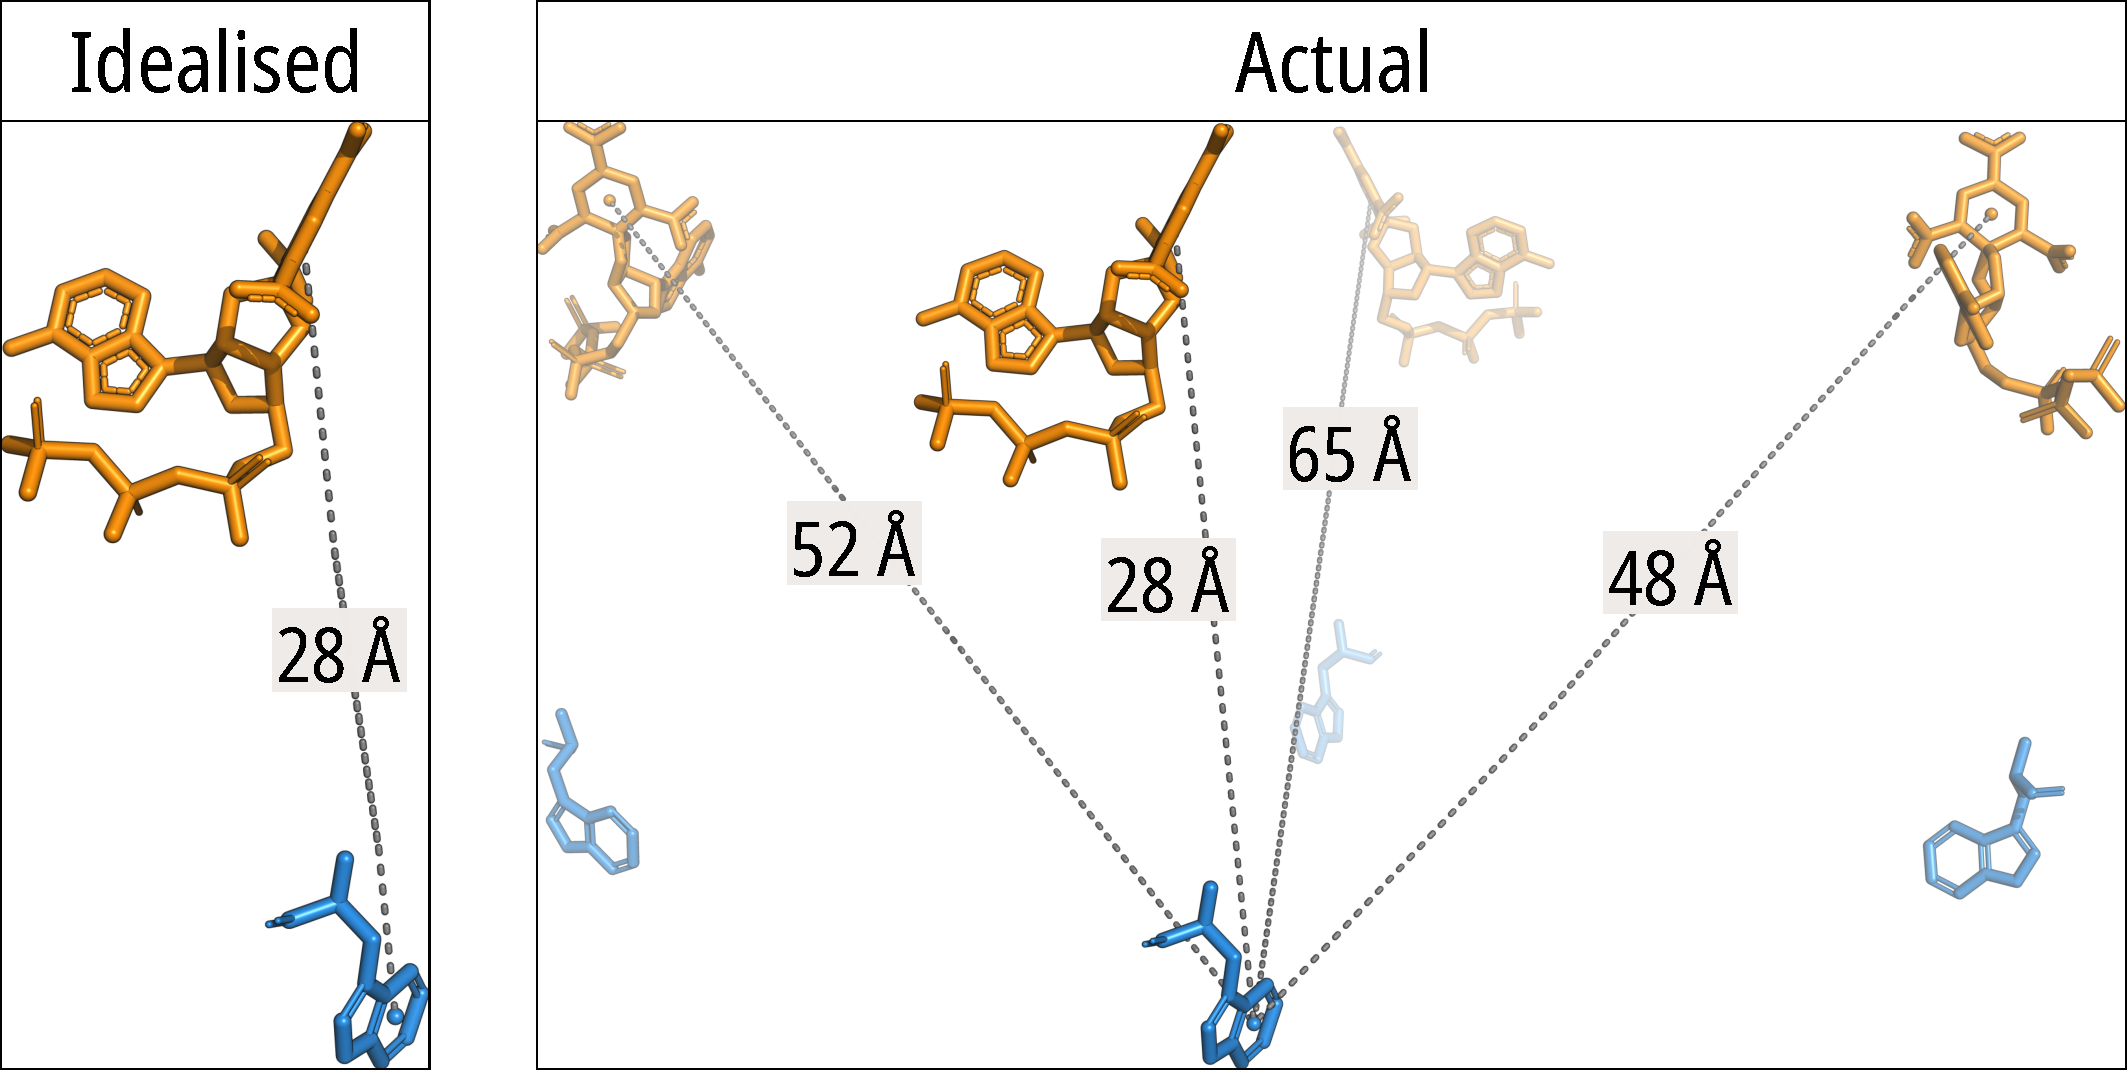
\includegraphics[width=\textwidth]{exifret_coords.pdf}
	\end{subfigure}
	\vfill
	\begin{subfigure}[t]{\textwidth}
		\caption{}\label{ch3fig:exifret_out}
		\centering
		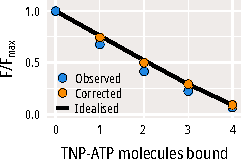
\includegraphics[width=\textwidth]{exifret_out.pdf}
	\end{subfigure}
	\end{minipage}
	\caption[Numerical analysis of FRET efficiency in tetrameric Kir6.2]{
	\subref{ch3fig:exifret_program} Schematic of the numerical simulation.
	After the geometry and fluorophore types are assigned, an exciton schedule is generated from the photon flux determined by the irradiance and wavelength of the LED used to excite ANAP.
	For each simulated photon (exciton), a relaxed donor is chosen at random.
	The donor releases its energy either via fluorescence or FRET to an acceptor based on the relative probability of each process.
	Donors and acceptors relax stochastically based on their fluorescence lifetimes (\SI{2}{\nano\second} for ANAP \cite{zagotta_measuring_2016-1} and \SI{0.05}{\nano\second} or \SI{2}{\nano\second} for TNP-ATP \cite{ye_spectroscopic_1999, ishikawa_single-molecule_2002}).
	Once the full exciton schedule is played, the total number of fluorescence and FRET events are summed and the total FRET efficiency is calculated.
	\subref{ch3fig:exifret_coords} Geometry of W311 and TNP-ATP molecules in tetrameric Kir6.2.
	W311 residues are from PDB \#6C3P, and TNP-ATP is from the highest scoring docking pose in Figure \ref{ch3fig:6c3p_docked}.
	Distances are measured from the centre of mass of the W311 sidechain to the centre of mass of each of the TNP moieties.
	\subref{ch3fig:exifret_out} Shown as a line is the idealised FRET efficiency for a single K\ATP{} channel bound to increasing numbers of TNP-ATP.
	Actual (blue) and corrected (orange) FRET efficiencies from the numerical simulation at each ligand occupancy state are shown as points.
	}
\end{figure}

Overall, these two corrections do not dramatically alter our results (Figure \ref{ch3fig:tnpatp_quenching_1}).
We observed quenching of ANAP fluorescence from W311*-GFP+SUR1 in unroofed membranes over a concentration range of TNP-ATP similar to the range in which we observed inhibition of current in excised patches expressing W311*-GFP+SUR1 (Figure \ref{ch3fig:tnpatp_quenching_2}).
When fit to a Hill equation, quenching ($F/F_{max}$) was fit with an EC\textsubscript{50} of \SIrange{21}{31}{\micro\Molar}, while the corrected binding data (adjusted $F/F_{max}$) gave an EC\textsubscript{50} of \SIrange{30}{45}{\micro\Molar}.

\begin{figure}[hbtp]
	\centering
	\begin{subfigure}[t]{0.8\textwidth}
		\caption{}\label{ch3fig:tnpatp_quenching_1}
		\centering
		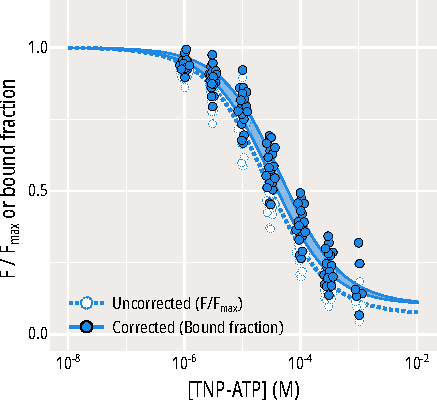
\includegraphics[width=\textwidth]{tnpatp_quenching_1.pdf}
	\end{subfigure}
	\vfill
	\begin{subfigure}[t]{0.9\textwidth}
		\caption{}\label{ch3fig:tnpatp_quenching_2}
		\centering
		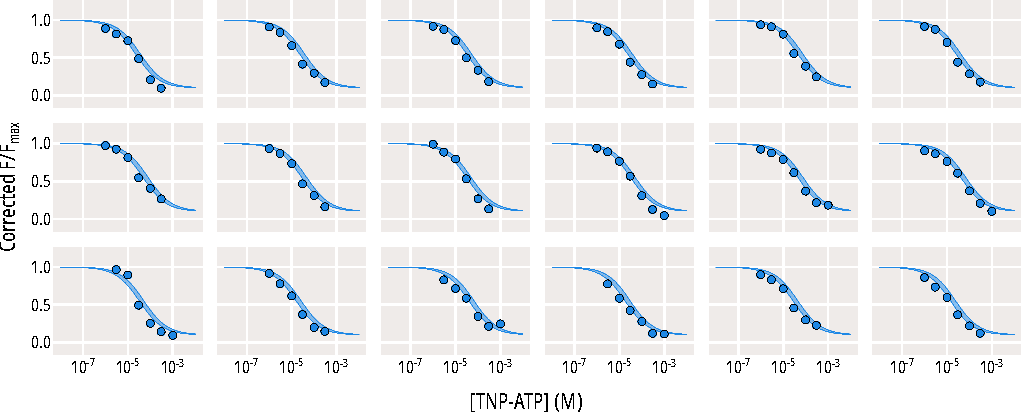
\includegraphics[width=\textwidth]{tnpatp_quenching_2.pdf}
	\end{subfigure}
	\caption[W311*-GFP unroofed membrane binding]{
	\subref{ch3fig:tnpatp_quenching_1} Fluorescence quenching of W311*-GFP+SUR1 by TNP-ATP in unroofed membrane patches.
	Each uncorrected point (white with blue outline) represents an individual measurement normalised to the maximum current observed in that unroofed membrane.
	Each corrected point (blue filled points) has been transformed to $log_2(\frac{F}{F_{max}}+1)$.
	The line is the median estimate and the smooth filled curves are the \SI{95}{\percent} credible intervals of the posterior probability distribution of fits to equation \ref{eq:hill} as described in the methods.
	The dashed curve is the median of the fits to the uncorrected data.
	\subref{ch3fig:tnpatp_quenching_2} Data from each experiment is shown separately.
	The smooth filled curves are the \SI{95}{\percent} credible intervals of the posterior predictions for each experiment.
	}
\end{figure}

\subsection{Patch-clamp fluorometry of Kir6.2 constructs}

To ensure that the ANAP fluorescence we observe in the unroofed membranes is emitted by functional channels, we measured fluorescence quenching and current inhibition from the same excised patches (Figure \ref{ch3fig:atp_tnpatp_trace}, \ref{ch3fig:atp_tnpatp_spectra_1}, \ref{ch3fig:atp_tnpatp_spectra_2}).
Notably, while ATP and TNP-ATP both inhibit K\ATP{} channel currents (Figure \ref{ch3fig:atp_tnpatp_trace}), we observe that ANAP fluorescence is only quenched by perfusion of TNP-ATP (Figure \ref{ch3fig:atp_tnpatp_spectra_2}).

This experimental paradigm leads to two complications compared to performing the measurements separately.
Firstly, the number of channels in an excised patch are far smaller than the number of channels in an unroofed membrane patch.
This results in a much dimmer fluorescence readout, and a lower signal-to-noise ratio.
Secondly, the presence of the pipette glass in the images results in some abnormalities in the background subtraction procedure.
This is not due to the glass itself, but results from the occlusion of TNP-ATP from the image surrounding the patch.
This leads to oversubtraction of the background TNP-ATP spectra, leading to an apparent negative peak in our corrected images.
However, we find that there is no overlap of this peak and the ANAP peak, so our fluorescence quenching measurements are unaffected by this phenomenon.
We were able to correct for ANAP bleaching in the same manner as we did for unroofed membranes (Figure \ref{ch3fig:pcf_bleaching}).

\begin{figure}[hbtp]
	\centering
	\begin{subfigure}[t]{0.9\textwidth}
		\caption{}\label{ch3fig:bleaching_plots_1}
		\centering
		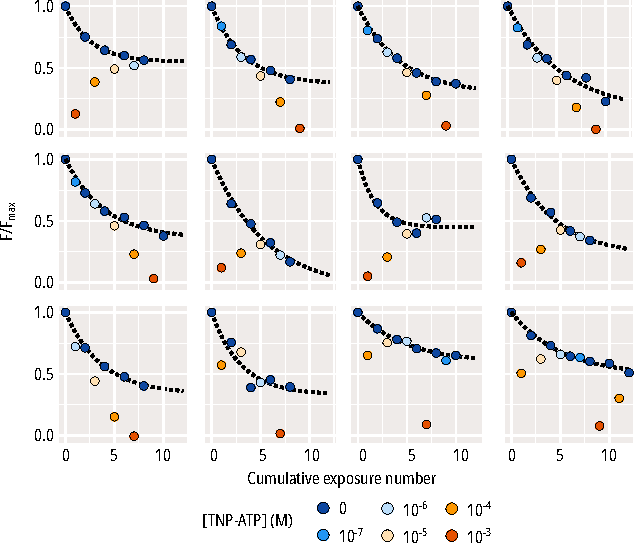
\includegraphics[width=\textwidth]{bleaching_plots_1.pdf}
	\end{subfigure}
	\vfill
	\begin{subfigure}[t]{0.45\textwidth}
		\caption{}\label{ch3fig:bleaching_terms_1}
		\centering
		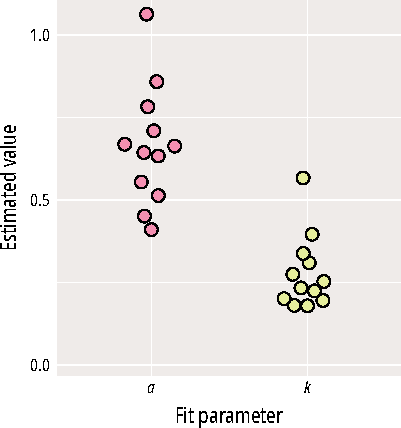
\includegraphics[width=\textwidth]{bleaching_terms_1.pdf}
	\end{subfigure}
	\hfill
	\begin{subfigure}[t]{0.45\textwidth}
		\caption{}\label{ch3fig:bleaching_terms_2}
		\centering
		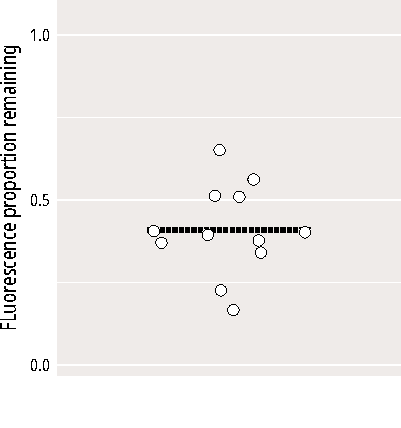
\includegraphics[width=\textwidth]{bleaching_terms_2.pdf}
	\end{subfigure}
	\caption[PCF bleaching correction]{
	\subref{ch3fig:bleaching_plots_1} Normalised ANAP fluorescence intensities in excised patches from cells expressing W311*-GFP+SUR1 perfused at different concentrations of TNP-ATP are shown as points coloured according to the concentration of TNP-ATP.
	The black dashed lines are fits to the fluorescence intensities without TNP-ATP present with equation \ref{eq:bleaching}.
	The order in which different TNP-ATP concentrations was applied varied between experiments.
	\subref{ch3fig:bleaching_terms_1} Values of the two parameters in equation \ref{eq:bleaching} for fits to each of the experiments in \subref{ch3fig:bleaching_plots_2}.
	\subref{ch3fig:bleaching_terms_2} Proportion of ANAP fluorescence remaining unbleached in the last exposure taken in the absence of TNP-ATP in each experiment.
	The dashed line is the mean, with a value of $0.41$.
	}\label{ch3fig:pcf_bleaching}
\end{figure}

Our fluorescence measurements from excised patches are right-shifted with respect to our measurements for unroofed membranes (Figure \ref{ch3fig:pcf_1}), with an $EC_{50}$ value of \SIrange{76}{144}{\micro\Molar} in PCF compared to \SIrange{30}{45}{\micro\Molar}.
Our finding that the EC\textsubscript{50} for TNP-ATP binding is right-shifted compared to the IC\textsubscript{50} for TNP-ATP inhibition is consistent between each experimental paradigm (Figure \ref{ch3fig:ec50_fits_4}).
This finding has implications for how exactly the binding of nucleotides to Kir6.2 leads to closure of the K\ATP{} channel pore.

\begin{figure}[hbtp]
	\centering
	\begin{subfigure}[t]{0.9\textwidth}
		\caption{}\label{ch3fig:atp_tnpatp_trace}
		\centering
		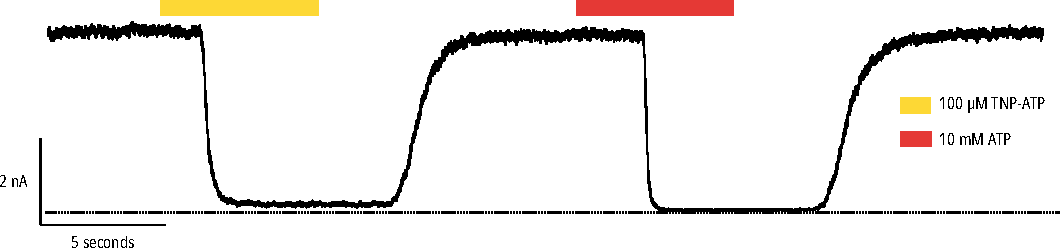
\includegraphics[width=\textwidth]{atp_tnpatp_trace.pdf}
	\end{subfigure}
	\vfill
	\begin{subfigure}[t]{0.5\textwidth}
		\caption{}\label{ch3fig:atp_tnpatp_spectra_1}
		\centering
		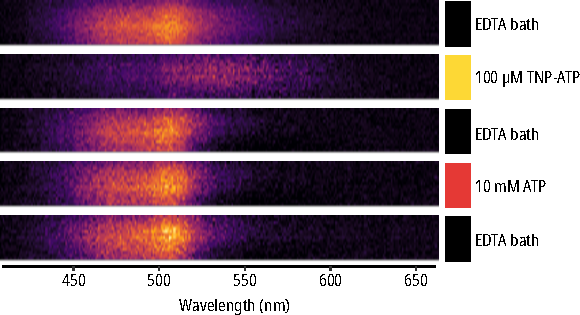
\includegraphics[width=\textwidth]{atp_tnpatp_spectral_images.pdf}
	\end{subfigure}
	\hfill
	\begin{subfigure}[t]{0.4\textwidth}
		\caption{}\label{ch3fig:atp_tnpatp_spectra_2}
		\centering
		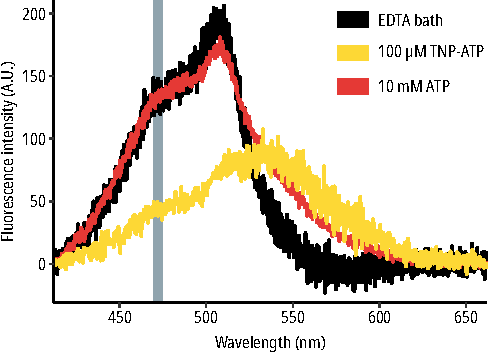
\includegraphics[width=\textwidth]{atp_tnpatp_spectral_traces.pdf}
	\end{subfigure}
	\vfill
	\begin{subfigure}[t]{0.45\textwidth}
		\caption{}\label{ch3fig:pcf_1}
		\centering
		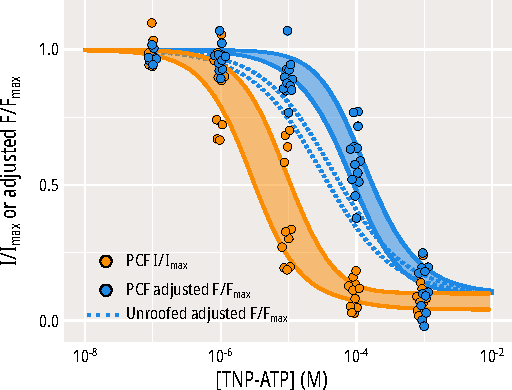
\includegraphics[width=\textwidth]{pcf_1.pdf}
	\end{subfigure}
	\hfill
	\begin{subfigure}[t]{0.45\textwidth}
		\caption{}\label{ch3fig:ec50_fits_4}
		\centering
		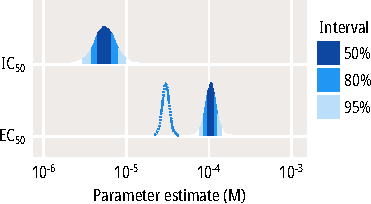
\includegraphics[width=\textwidth]{ec50_fits_4.pdf}
	\end{subfigure}
	\caption[ANAP is not quenched by ATP]{
	\subref{ch3fig:atp_tnpatp_trace} Current trace from an excised patch expressing W311*-GFP+SUR1 perfused with either ATP or TNP-ATP.
	The zero current level is shown as a dotted line, and the nucleotide applications are marked as coloured bars.
	\subref{ch3fig:atp_tnpatp_spectra_1} Spectra captured from the same patch during the nucleotide applications marked in \subref{ch3fig:atp_tnpatp_trace}, and during the washout periods between applications.
	Each spectra was captured with a one second exposure and corrected for background fluorescence and bleaching as described in the main text.
	The location of the three fluorescent peaks are indicated by arrows at the top of the plot.
	\subref{ch3fig:atp_tnpatp_spectra_2} Averaged traces of the spectra shown in \subref{ch3fig:atp_tnpatp_spectra_1}.
	The three fluorescence peaks are maked with shaded blue (ANAP), green (GFP) and orange (TNP-ATP) bars.
	\subref{ch3fig:pcf_1} Current inhibition ($I/I_{max}$, orange points) and fluorescence quenching (adjusted $F/F_{max}$, blue points) of W311*-GFP+SUR1 in excised membrane patches recorded simultaneously.
	The line is the median estimate and the smooth filled curves are the \SI{95}{\percent} credible intervals of the posterior probability distribution of fits to equation \ref{eq:hill} as described in the methods.
	The dashed blue line is the median fit to the fluorescence quenching in unroofed membranes reported in Figure \ref{ch3fig:tnpatp_quenching_1}.
	\subref{ch3fig:ec50_fits_4} Posterior probability distributions for the estimated population $EC_{50}$ and $IC_{50}$ values are shown coloured according to their credible intervals.
	The posterior probability distribution for the $EC_{50}$ values in unroofed membranes is derived from the data in Figure \ref{ch3fig:tnpatp_quenching_1}.
	}\label{ch3fig:pcf_intro_1}
\end{figure}

\section{Discussion}

We have demonstrated that we can measure nucleotide binding to the inhibitory nucleotide binding site of Kir6.2 in intact, functional K\ATP{} channels in their native membrane environment.
Measuring binding directly in either unroofed membrane patches, or in excised patches simultaneously with current recordings, reveals that nucleotide binding is right-shifted compared to nucleotide inhibition; i.e. K\ATP{} channels begin to close at nucleotide concentrations where there is very little binding.
This observation rules out certain models of ion channel function, which will be explored further in chapter \ref{ch:4}.

These findings come with some important caveats.
Firstly, the introduction of ANAP into Kir6.2 at residue 311 clearly impacts nucleotide inhibition of the channel, increasing the observed $IC_{50}$ values for ATP.
Our analysis of nucleotide binding and inhibition is therefore predicated on this decrease in sensitivity to ATP inhibition not reflecting a disruption of the normal physiological mechanism of ATP inhibition.
As all of our binding experiments are performed in the W311* background by necessity, we hope that measurements of relative changes in binding and inhibition will still be meaningfuly interpretable as they will mirror similar relative changes in inhibition observed in the WT background.

Secondly, K\ATP{} channels are more sensitive to inhibition by TNP-ATP than by ATP.
Again, this means that any conclusions we draw from experiments measuring relative changes in binding and inhibition rely on those relative changes affecting ATP binding and inhibition to a similar extent as TNP-ATP.
To try and ameliorate these caveats as best as we can, where possible we have performed control experiments in the WT background with ATP to ensure that introduced mutations result in similar relative effects on nucleotide inhibition despite the background of the construct or the identitity of the nucleotide.
As control experiments of this sort are not possible in unroofed membranes, where it is impossible to measure current inhibition, we have focused on PCF for constructs where expression is good enough to measure sufficient fluorescence.

Finally, there is a clear difference between the $EC_{50}$ values we estimate from TNP-ATP binding in unroofed membranes and in excised patches.
This may be due to increased levels of channel rundown in unroofed membranes, as the time between unroofing and measurement is longer (not measured, but around 10 minutes until first exposure) than the time between patch excision and measurement (typically less than a minute before first exposure).
Rundown K\ATP{} channels with a lower $P_O$ would be expected to have lower apparent $EC_{50}$ values for TNP-ATP binding.
An additional possibility is that our unroofing procedure does not result in all of the cell contents being disrupted, and that some of the ANAP fluorescence we are measuring is from W311*-GFP subunits resident in ER fragments associated with the adherent membrane.
Again, where possible we have tried to perform our experiments with PCF to avoid these possibilities.
